\documentclass[15pt,a4paper]{article}
\pdfoutput=1

%=========================Package begin========================%
\usepackage{amsmath}
\usepackage{color}
\usepackage{cite}               % citiation
\usepackage{float}
\usepackage{graphicx, subfig}
\usepackage{geometry}
\usepackage{caption}
\usepackage{indentfirst}
\usepackage{times}              % set Times New Romans type
\usepackage{setspace}           % set line to line space 
%=========================Package end========================%
\geometry{left=2.5cm,right=2.5cm,top=2.5cm, bottom=2.5cm}

\title{\textbf{LOCld55 Design Document}}

%Email:wzhang@mails.ccnu.edu.cn

\author{\textbf{Author:} Wei Zhang, Di Guo, Quan Sun}

%\affil{College}
\date{\today}

\begin{document}
\begin{spacing}{1.25}           % set line to line space is 1.25
\maketitle


\thispagestyle{empty}           % first page doesn't page number

\newpage

\tableofcontents                % Create contents

\thispagestyle{empty}           % second page doesn't page number

\newpage

\setcounter{page}{1}

\section{General Description of LOCld55}    % Part One

LOCld55 is a \textbf{single-channel, 14Gbps VCSEL driver} ASIC designed under SMIC 55nm CMOS technology specifically for datacom and telecommunication applications. The design follows the references\cite{ref1}.

Figure 1 illustrates the block diagram of LOCld55 that includes a laser driver, I2C control unit, and limiting amplifier receiver.

%Figure 1: LOCld55 block diagram
\begin{figure}[H]
    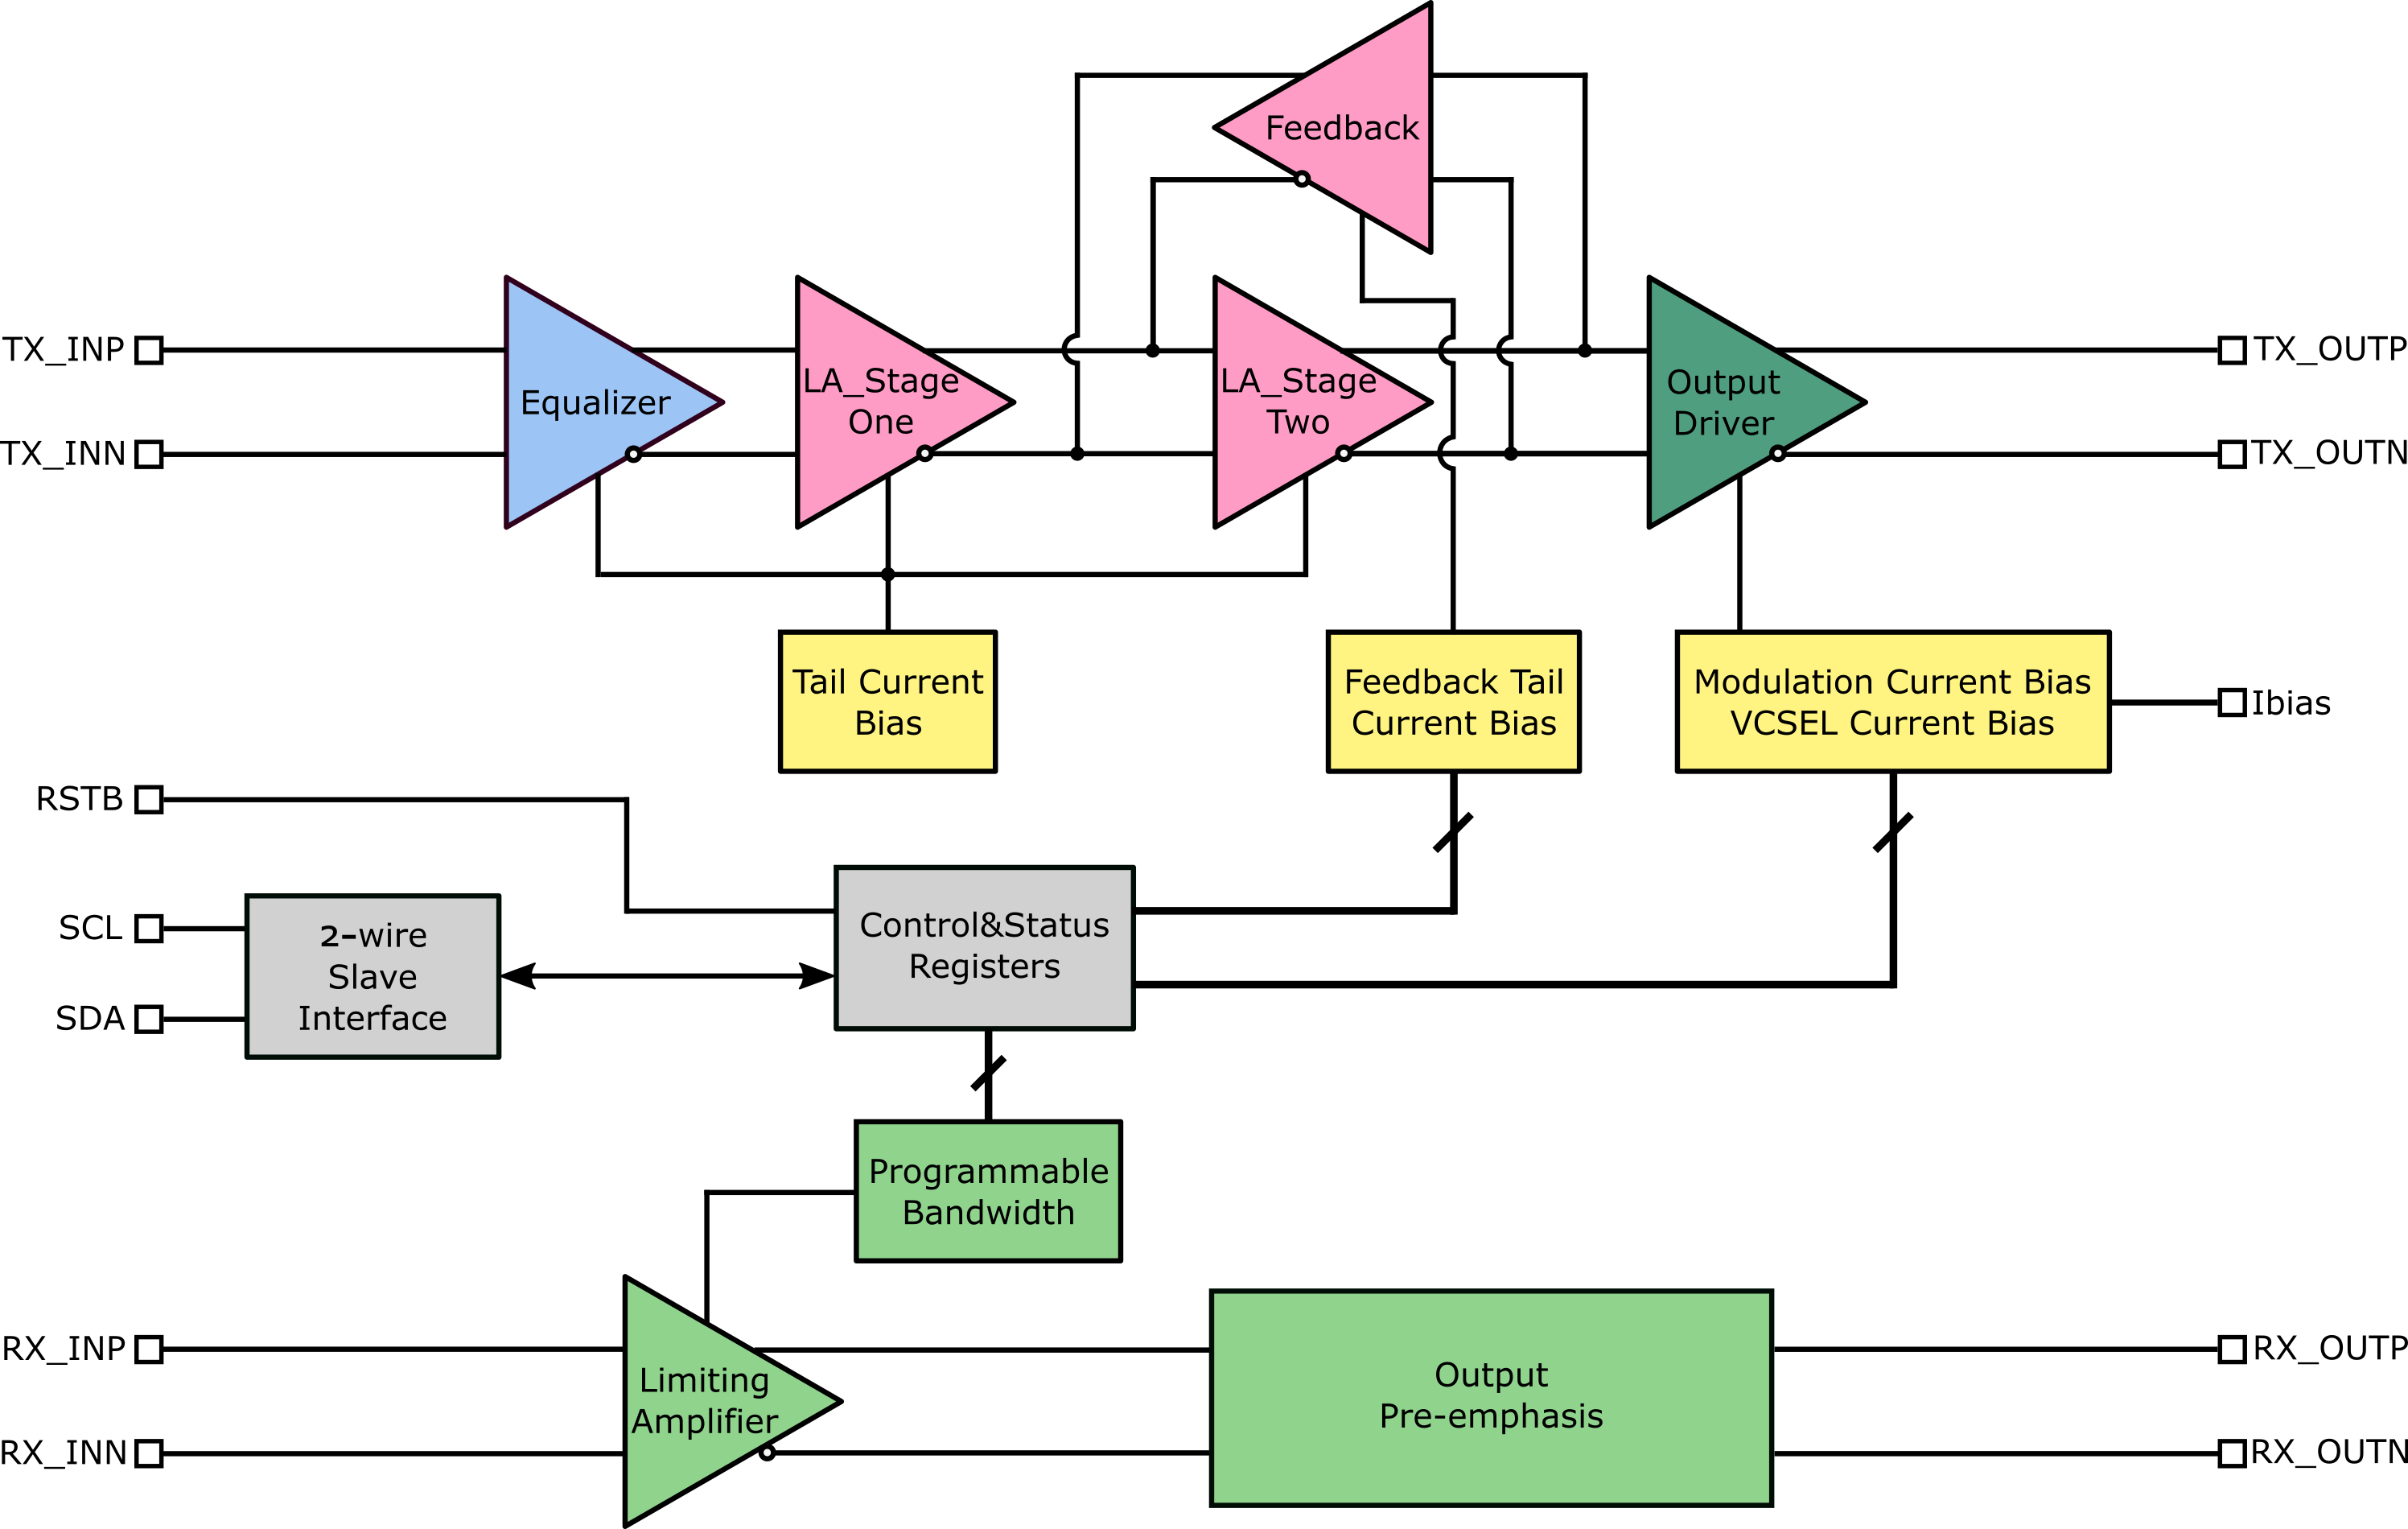
\includegraphics[width=\linewidth]{./Img/locld55.png}
    \caption{LOCld55 block diagram}
%    \lable{Figure 1}
\end{figure}
%Figure 1: LOCld55 block diagram

The die size and pad out of LOCld55 are shown in Section 2. Detailed schematic and layout designs are discussed in Section 3. The post-layout simulation results are introduced in Section 4.

\section{Pin Out of LOCld55}                % Part Two 

\subsection{Pin Assignment}

\subsection{Pin Descriptions}

\section{Detailed design of LOCld55}        % Part Three
\subsection{Equalizer}

\subsection{Limited Amplifier (LA)}

\subsection{Output Driver (OD)}

\subsection{Equalizer and Limited Amplifier biasing circuit}

\subsection{Modulation biasing circuit and Current biasing circuit}

\subsection{I2C}

\section{LOCld55 simulation results}        % Part Four

\subsection{Equalizer simulation results}

\subsection{Limiting Amplifier simulation results}

\section{References}                        % Part Five

\end{spacing}

\bibliographystyle{plain}
\bibliography{LOCld55_Design_Document}


\end{document}
